Al hacer click en el siguiente botón:

\begin{figure}[H]
    \centering
    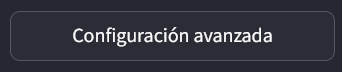
\includegraphics[width=\textwidth,height=0.16\textheight,keepaspectratio]{commons/BotonConfig_GUI.png}
    \caption{Botón de configuración.}
    \label{fig:boton-config-gui-1}
\end{figure}

El sistema lleva al usuario a una nueva pantalla donde se pueden modificar los hiperparámetros del modelo:

\textbf{Parámetros de la formación de transformadas de Fourier}

\begin{figure}[H]
    \centering
    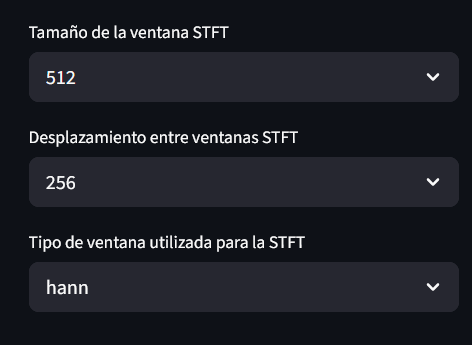
\includegraphics[width=\textwidth,height=0.16\textheight,keepaspectratio]{commons/ParamsSTFT_GUI.png}
    \caption{Parámetros de formación de transformadas de Fourier modificables en la interfaz visual.}
    \label{fig:params-stft-gui}
\end{figure}

\textbf{Parámetros intrínsecos modelo}

\begin{figure}[H]
    \centering
    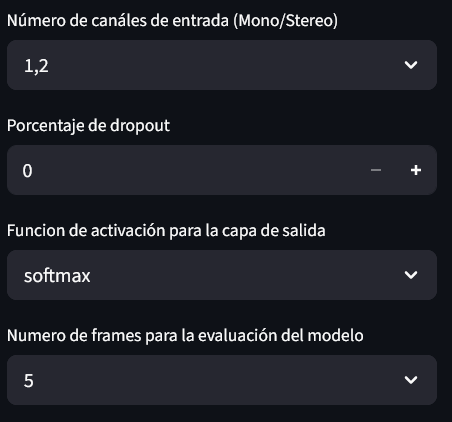
\includegraphics[width=\textwidth,height=0.16\textheight,keepaspectratio]{commons/ParamsModelo_GUI.png}
    \caption{Parámetros intrínsecos del modelo modificables en la interfaz visual.}
    \label{fig:params-modelo-gui}
\end{figure}

\textbf{Parámetros de entrenamiento}

\begin{figure}[H]
    \centering
    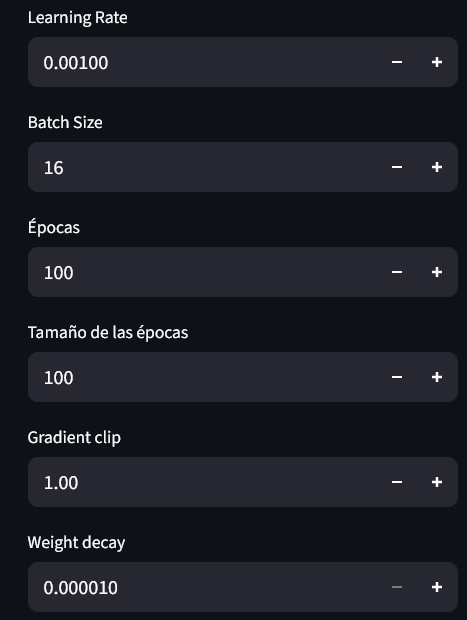
\includegraphics[width=\textwidth,height=0.16\textheight,keepaspectratio]{commons/ParamsEntrenamiento_GUI.png}
    \caption{Parámetros modificables de entrenamiento de nuevos modelos en la interfaz visual.}
    \label{fig:params-train-gui}
\end{figure}

\textbf{Parámetros de efectos para entrenamiento y de audio}

\begin{figure}[H]
    \centering
    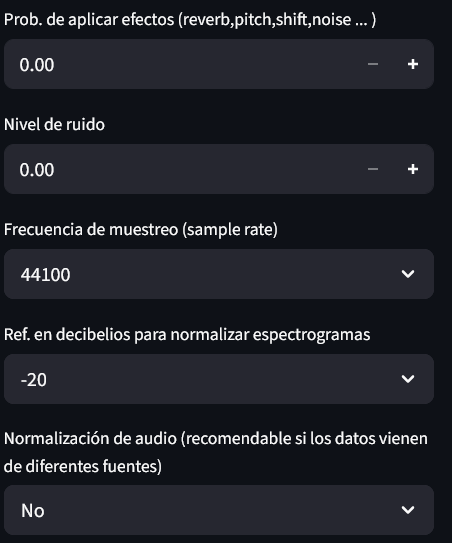
\includegraphics[width=\textwidth,height=0.16\textheight,keepaspectratio]{commons/ParamsEfectos_GUI.png}
    \caption{Parámetros modificables de generación de efectos en la interfaz visual.}
    \label{fig:params-efectos-gui}
\end{figure}

\textbf{Parámetros de generación de mezclas}

\begin{figure}[H]
    \centering
    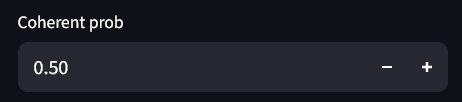
\includegraphics[width=\textwidth,height=0.16\textheight,keepaspectratio]{commons/ParamsMezclas_GUI.png}
    \caption{Parámetros modificables de generación de mezclas en la interfaz visual.}
    \label{fig:params-generacion-gui}
\end{figure}